\documentclass[fleqn]{article}

\usepackage{mydefs}
\usepackage{notes}
\usepackage{url}
\usepackage{graphicx}

\begin{document}
\lecture{CS4400}{Problem Set 14}{Alex Clemmer, u0458675}

\section*{12.25}

Reentrant and threadsafe. The only possibly-troublesome variables are \texttt{mutex} (handled properly) and \texttt{once} (also handled properly. Everything else is locked down by the mutex.

\section*{12.28}

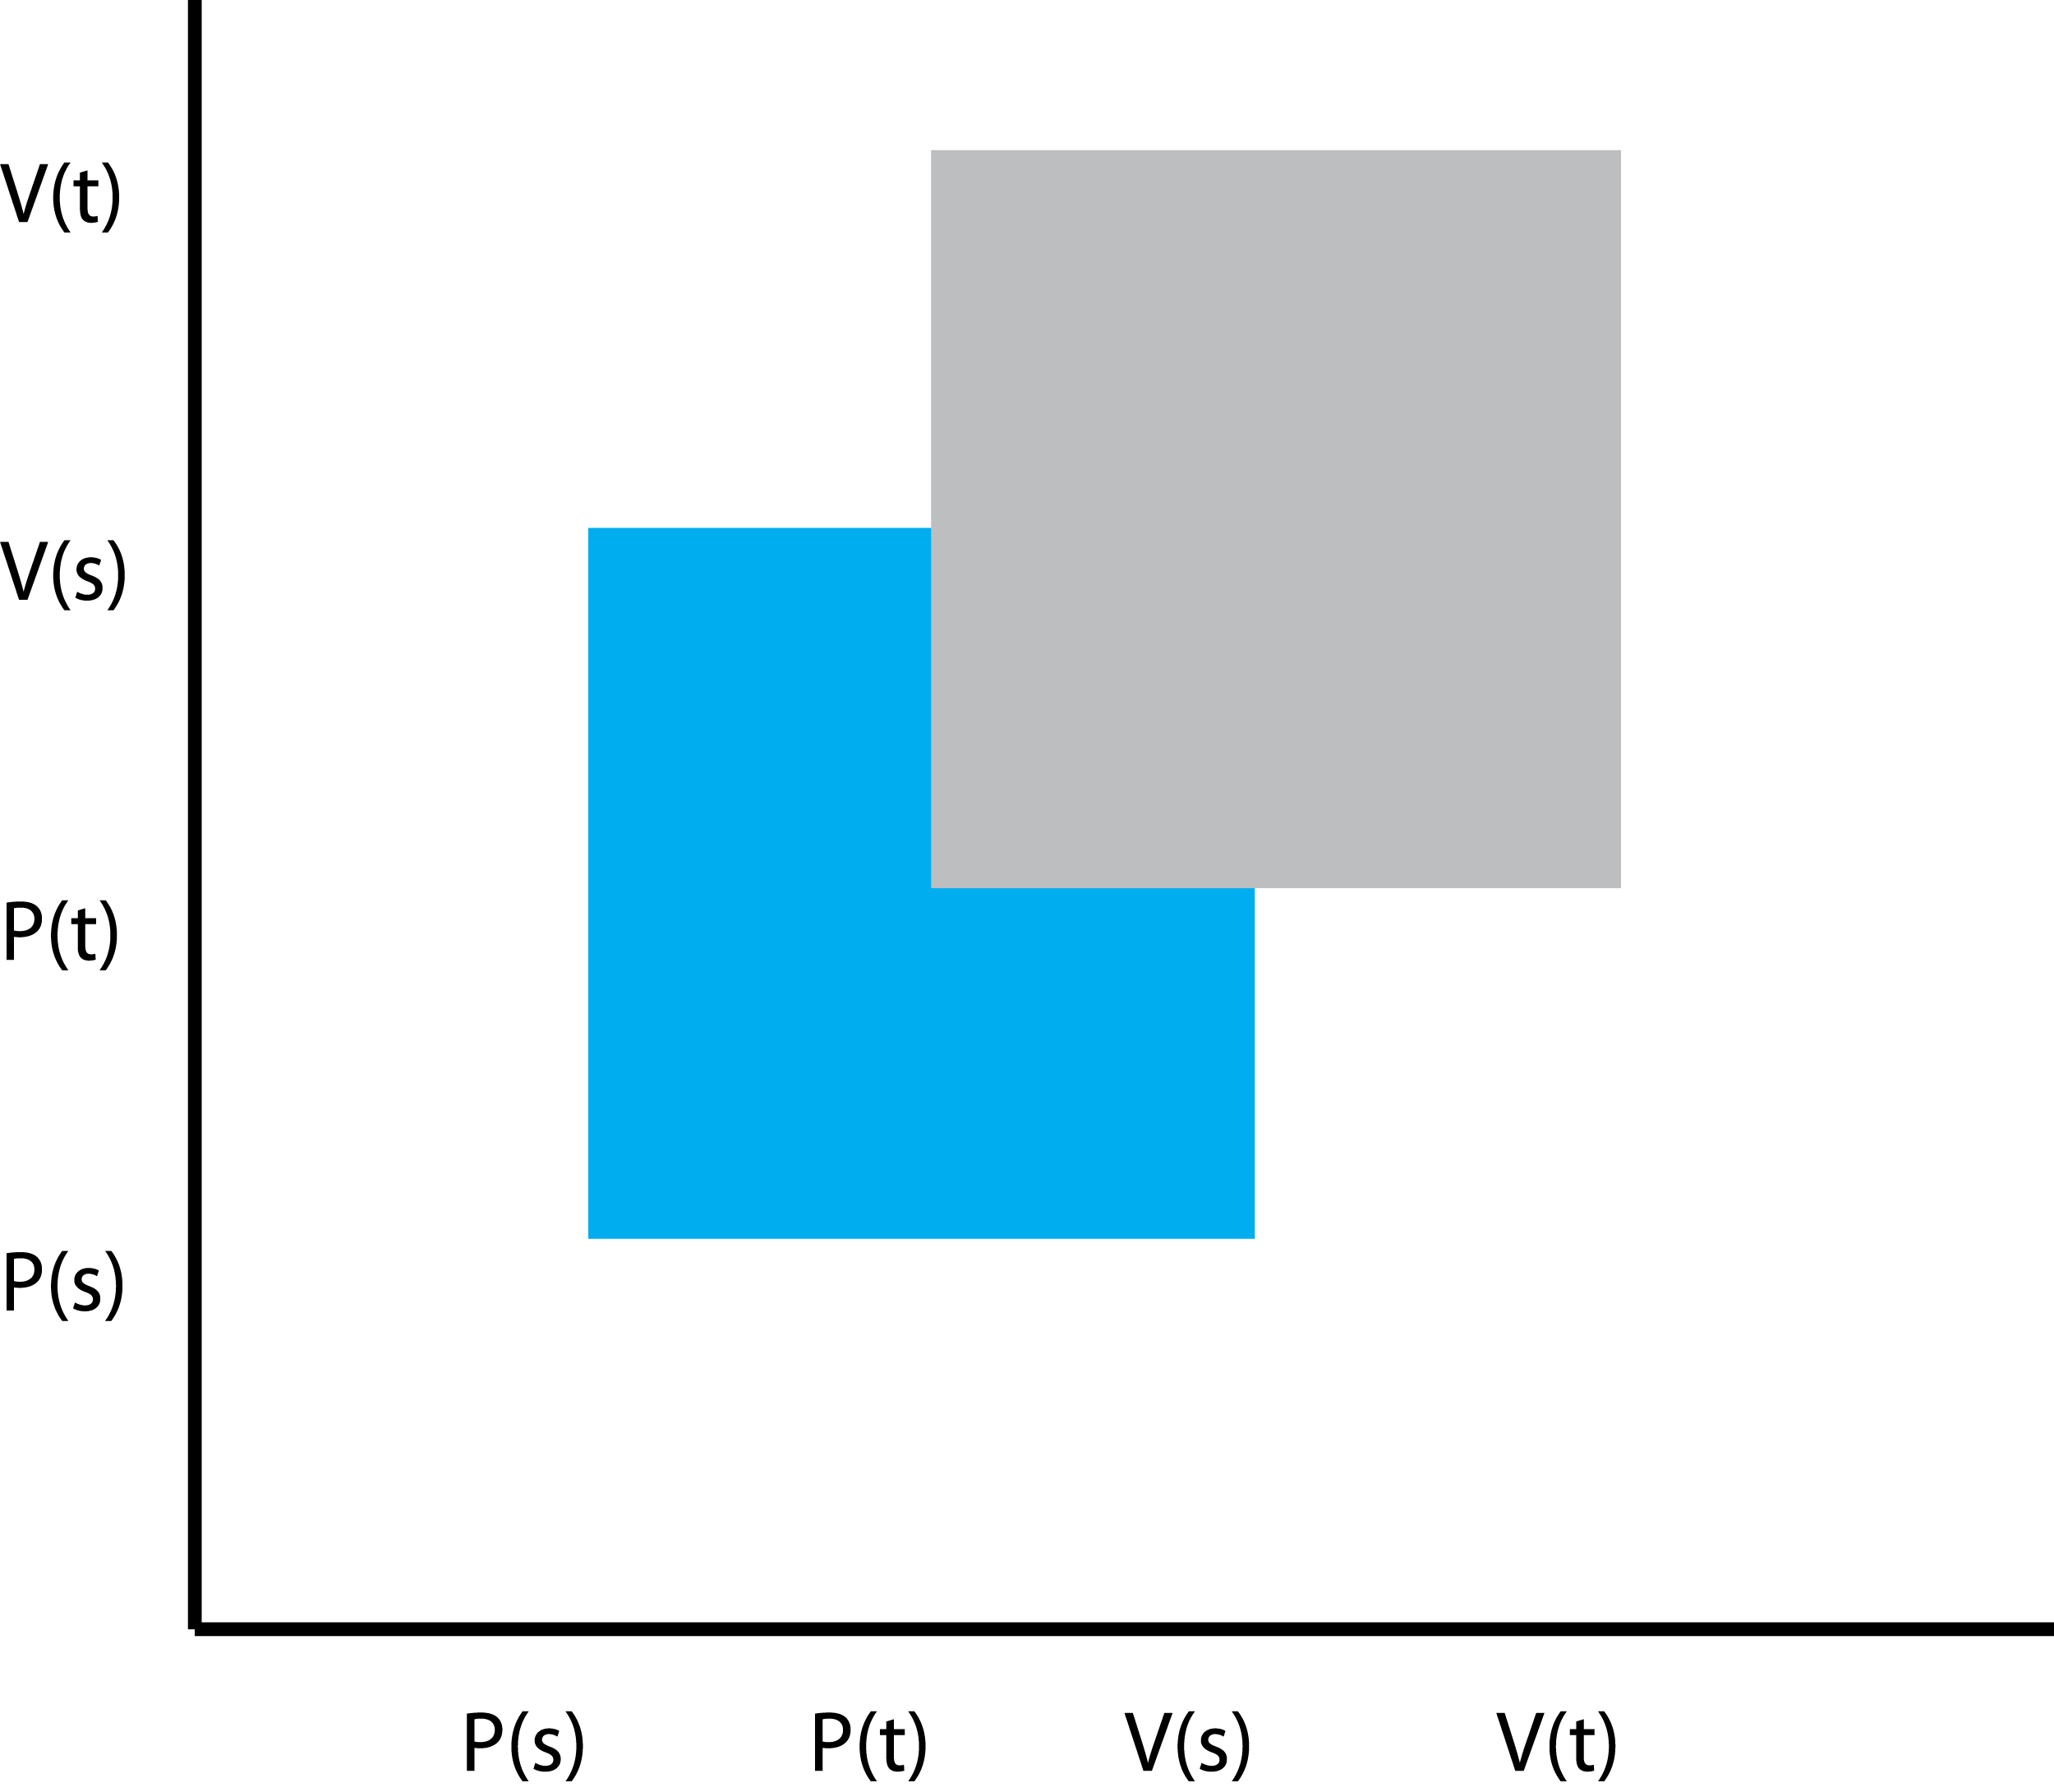
\includegraphics[scale=0.25]{1.png}
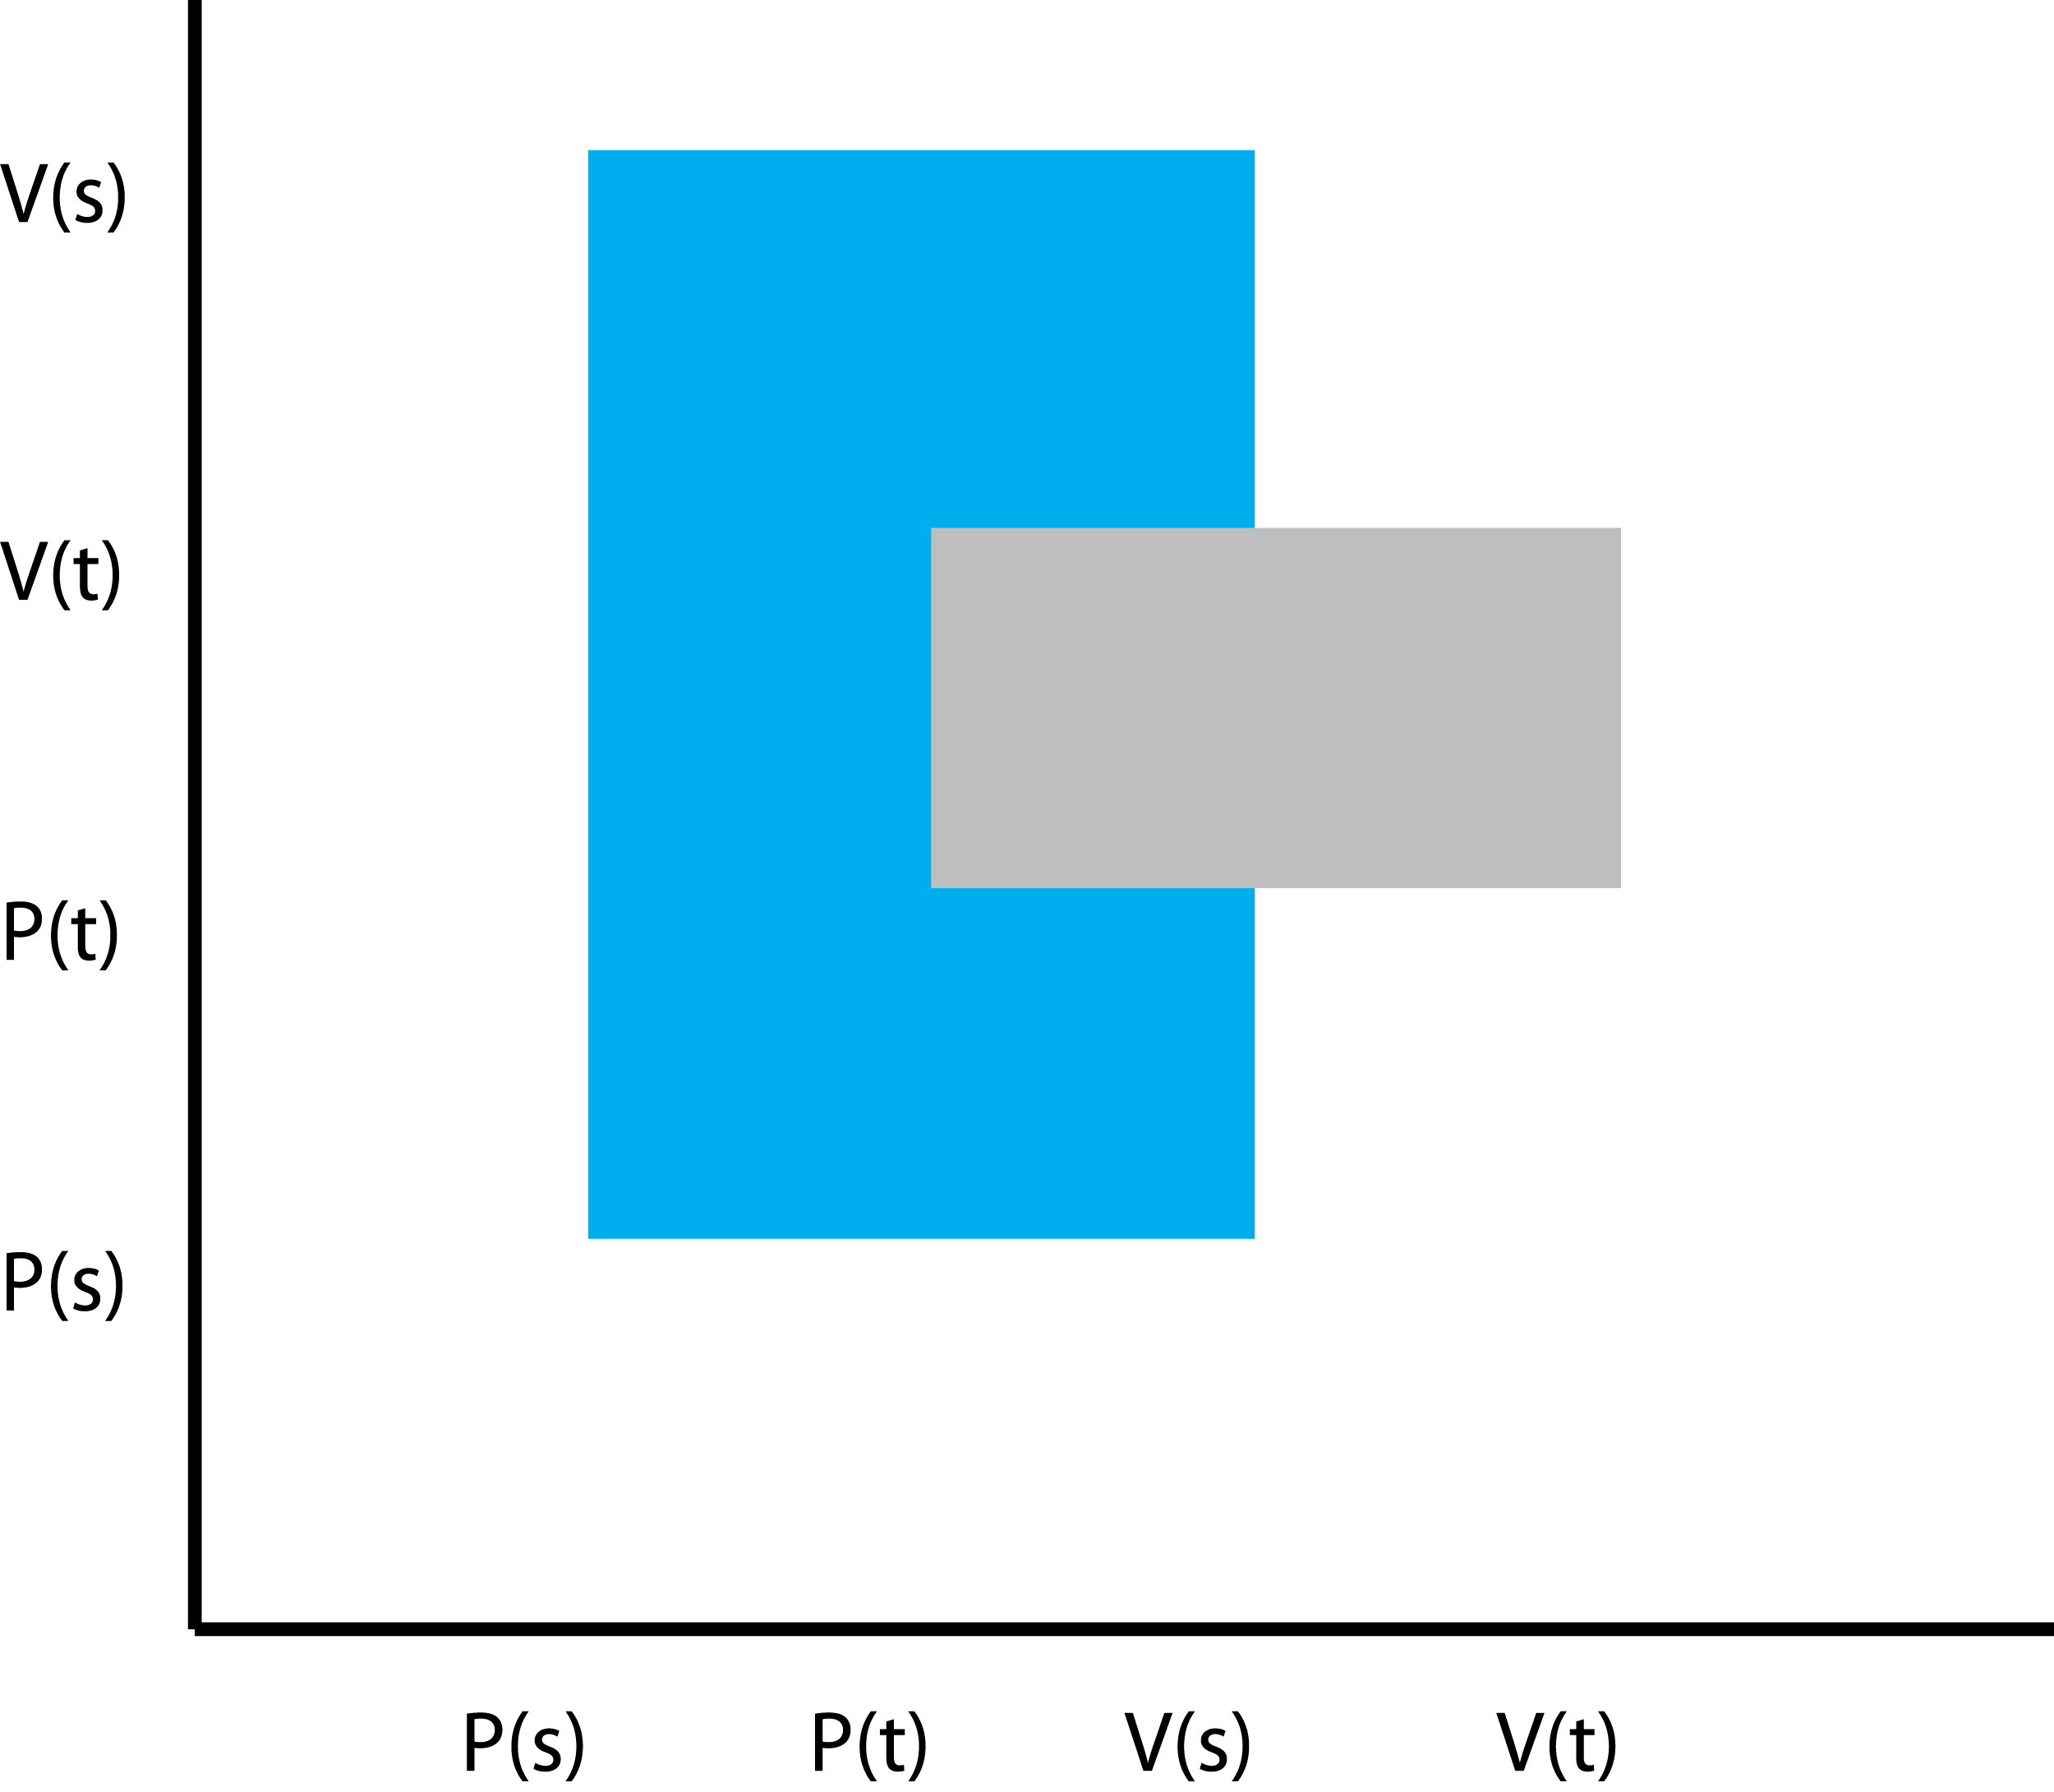
\includegraphics[scale=0.25]{2.png}
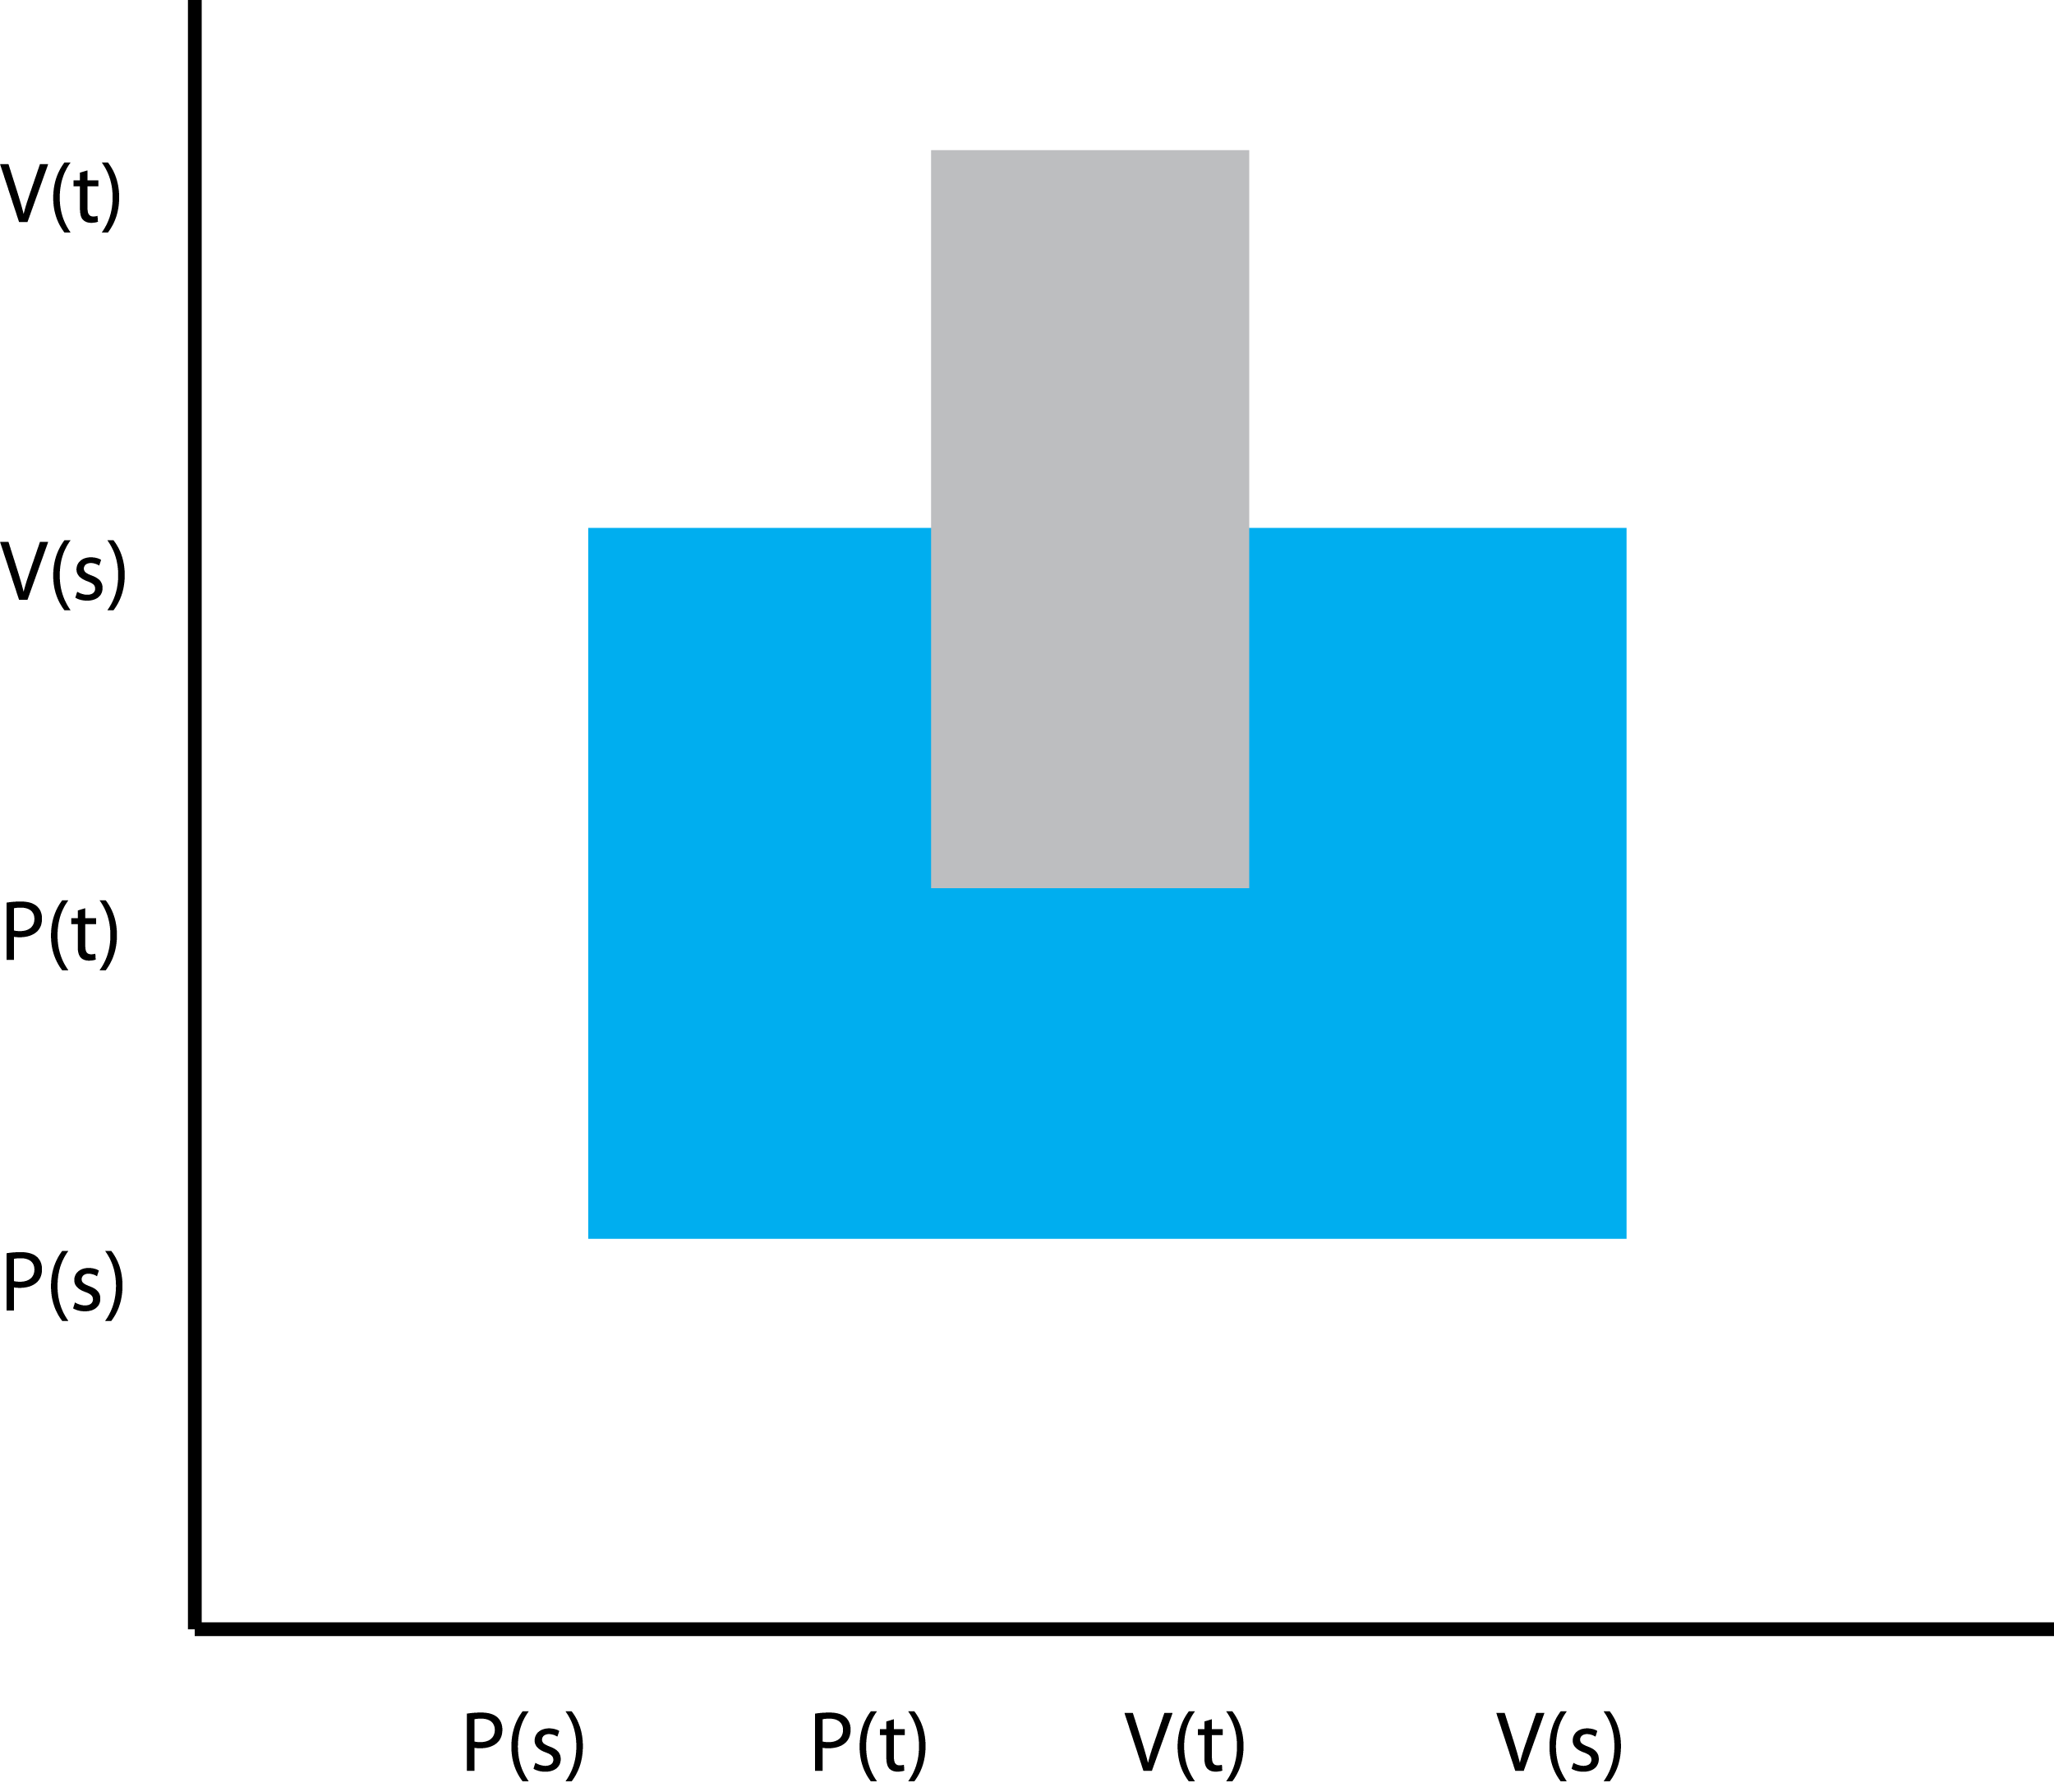
\includegraphics[scale=0.25]{3.png}
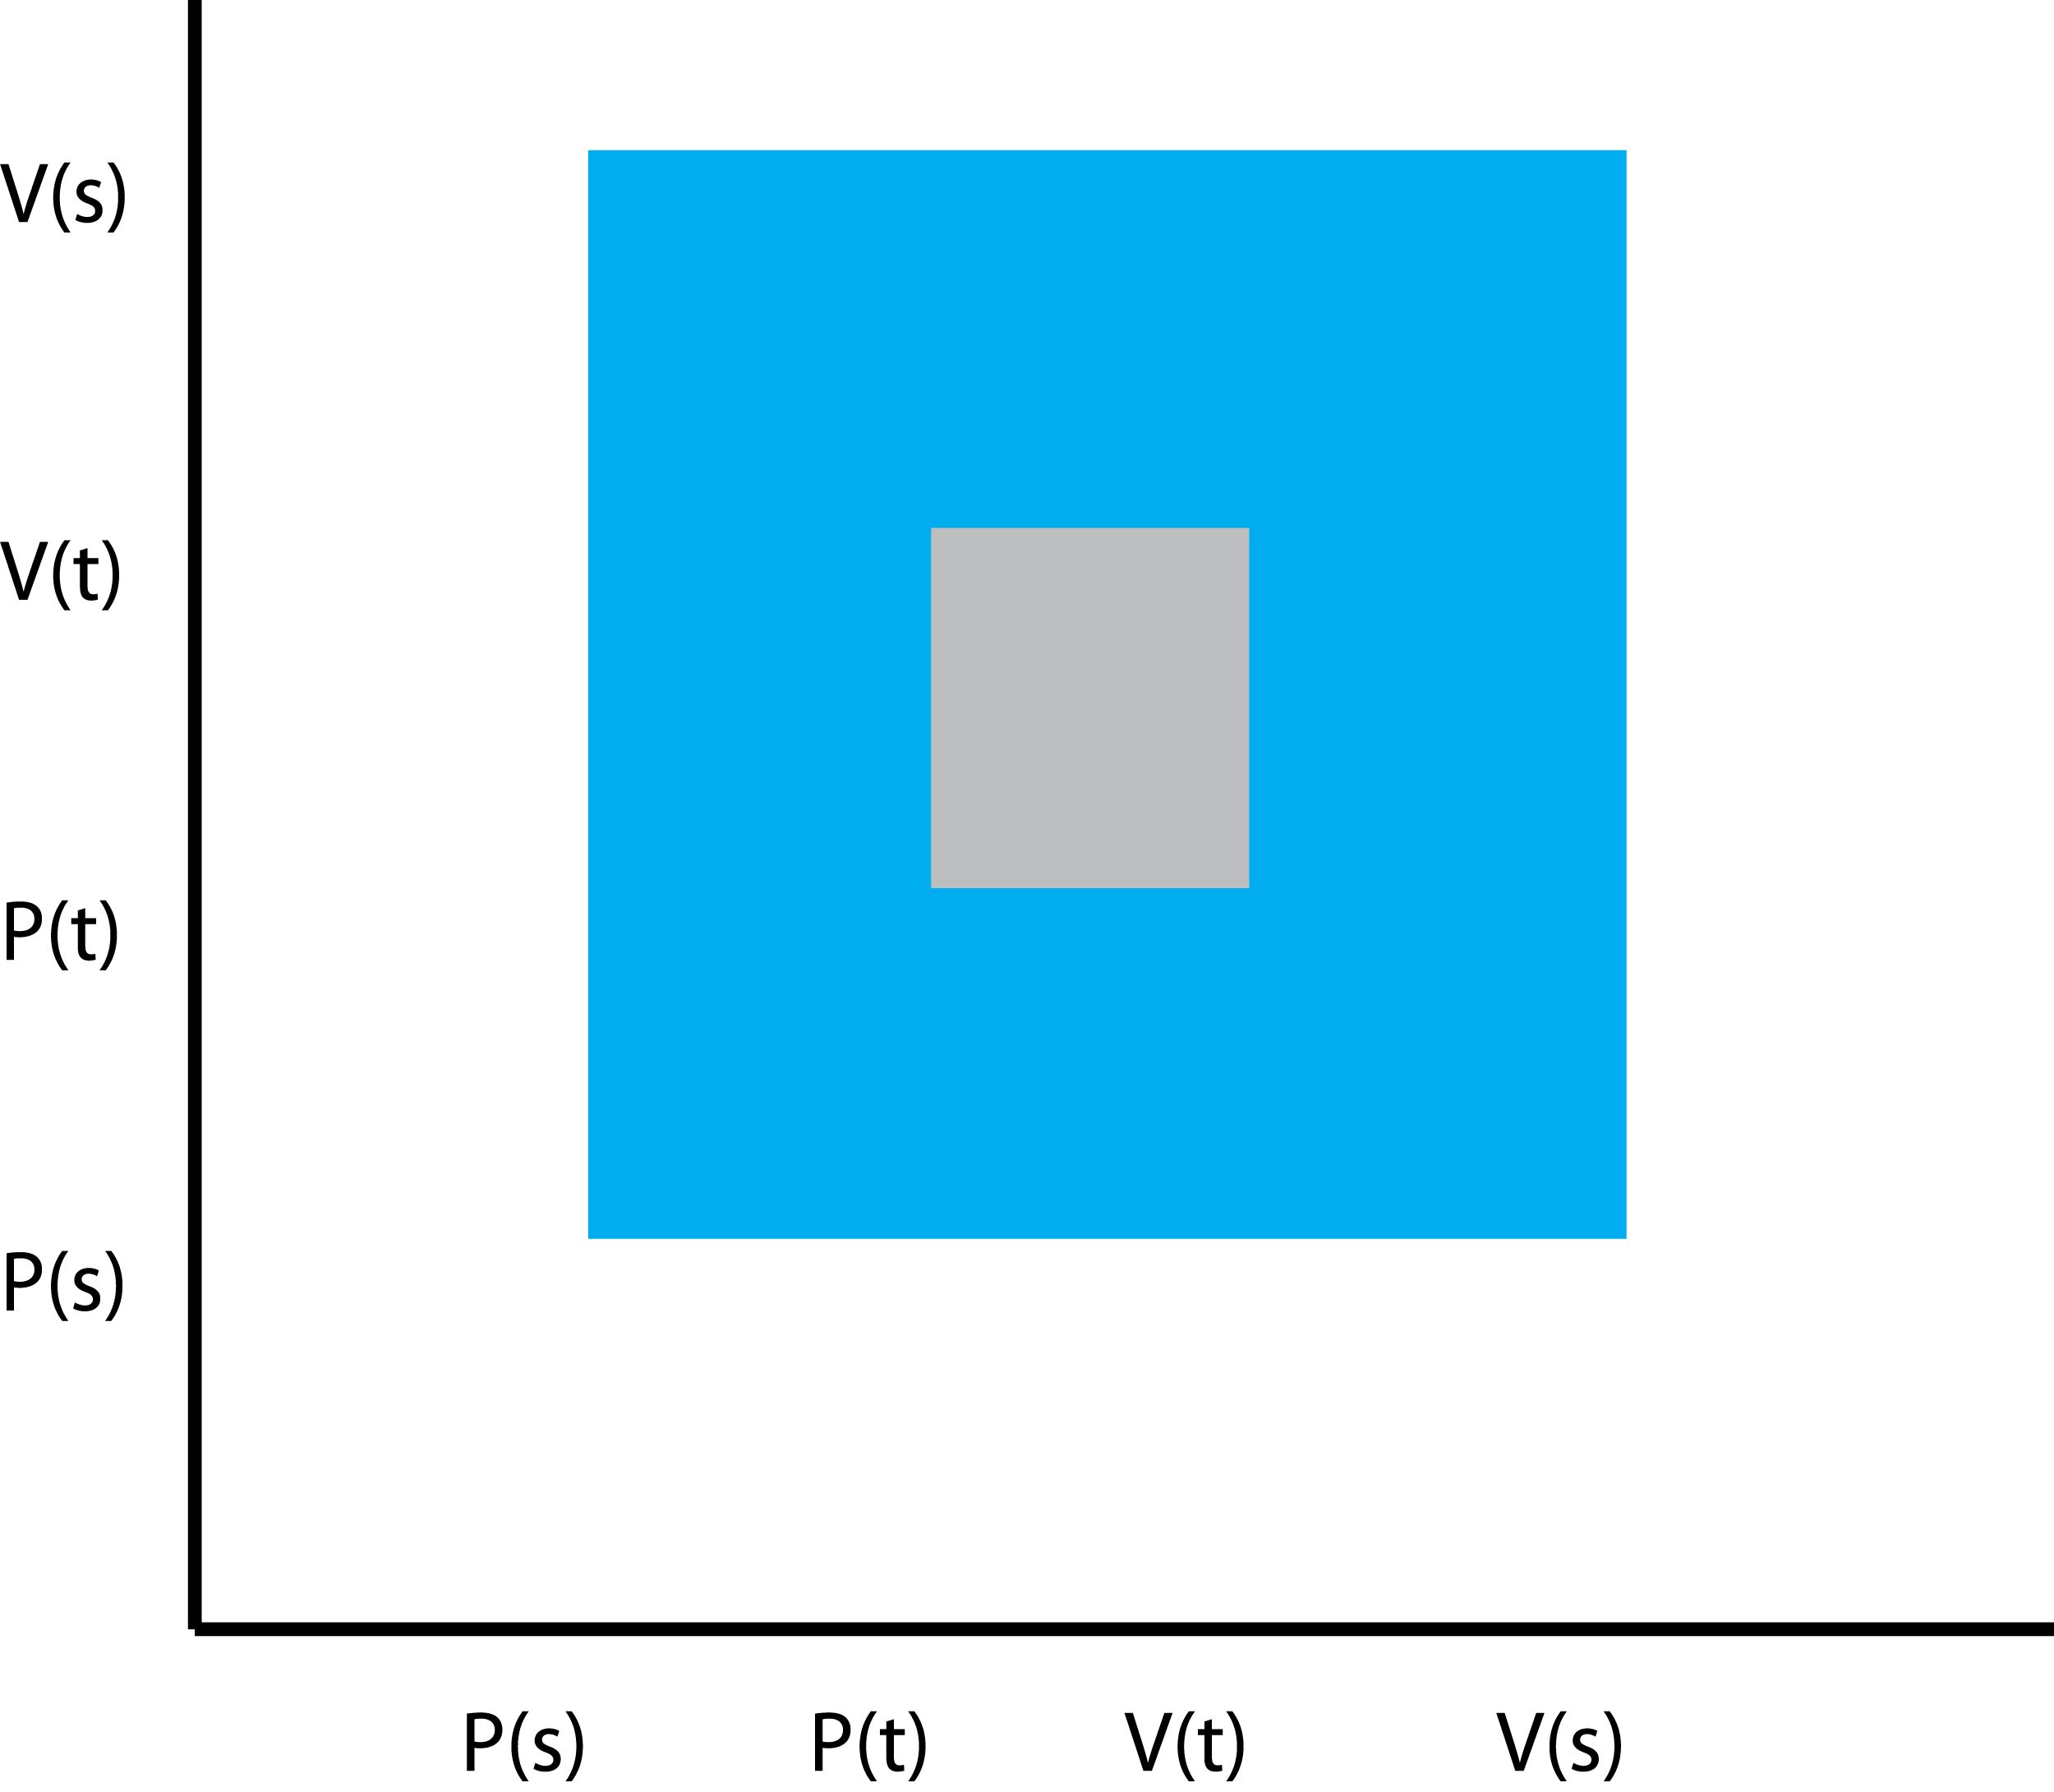
\includegraphics[scale=0.25]{4.png}

\section*{12.29}

No it cannot. Thread 1 occurrs entirely sequentially with the one exception of \texttt{a}, which encapsulates everything. Since thread 2 doesn't use \texttt{a}, so deadlock is not possible there. In thread 2, \texttt{b} is nested in \texttt{a}, but in thread 1, there is no other nesting, so it impossible for both threads to just wait for the other to release the lock.

\end{document}
